\documentclass[11pt, a4paper, reqno]{scrartcl}

\usepackage[utf8]{inputenc}
\usepackage{a4wide}
\usepackage{libertine}
\usepackage{graphicx}
\usepackage{listings}
\usepackage{xcolor}
\usepackage{float}
\usepackage{amsmath}
\usepackage{microtype}
\usepackage{hyperref}
\usepackage{pdflscape}

% for latex output of pandas
\usepackage{booktabs}

\begin{document}
    \title{Exercise No. 3}
    \author{David Bubeck, Pascal Becht, Patrick Nisbl\`e}
    \maketitle

    \lstset{
        language=Python,
        backgroundcolor=\color{gray!5},
        numbers=left,
        captionpos=t,
        breaklines=true,
        frame=l,
        xleftmargin=\parindent,
        basicstyle=\footnotesize\sffamily,
        keywordstyle=\bfseries\color{green!40!black},
        commentstyle=\itshape\color{purple!40!black},
        identifierstyle=\color{blue!60!black},
        stringstyle=\color{orange}
    }

    \section{2 - Three Body System}
    \subsection{a)}
    
        Problem: Simulate a three-body system with given initial positions and velocities ($y_1$ to $y_{12}$) using the Runge-Kutta-Scheme of 4th order\\\\        
        Using the following implementation of the RK4 method:
        \begin{figure}[H]
            \lstinputlisting[lastline=27, firstline=7, firstnumber=7]{rk4.py}
            \caption{rKN-function for iterative use on previous calculated values}
        \end{figure}
        and the following set of equations:
        \begin{align}
            \dot {\overrightarrow{x_{n+1}}} =& \vec v_{n}\\
            \dot {\overrightarrow{v_{n+1}}} =& \frac{G m_2}{r_{12,n}^2}\frac{\vec r_{12,n}}{r_{12,n}} + \frac{G m_3}{r_{13,n}^2}\frac{\vec r_{13,n}}{r_{13,n}}
        \end{align}
        where $r_n = \| \vec r\|$, for $m_1$
        
        \begin{figure}[H]
            \lstinputlisting[lastline=56]{rk4-threebody.py}
        \end{figure}
        \begin{figure}[H]
            \lstinputlisting[firstline=57, firstnumber=57]{rk4-threebody.py}
            \caption{implementation of a three-body system using the RK4 method}
        \end{figure}
        where when done for stepsizes between 0.01 and 0.001 we can only see a difference in calulated length over multiple steps, when accounted for stepsize the calculated paths look alike. 
        An animation was also created.
        \begin{landscape}
            \begin{figure}
                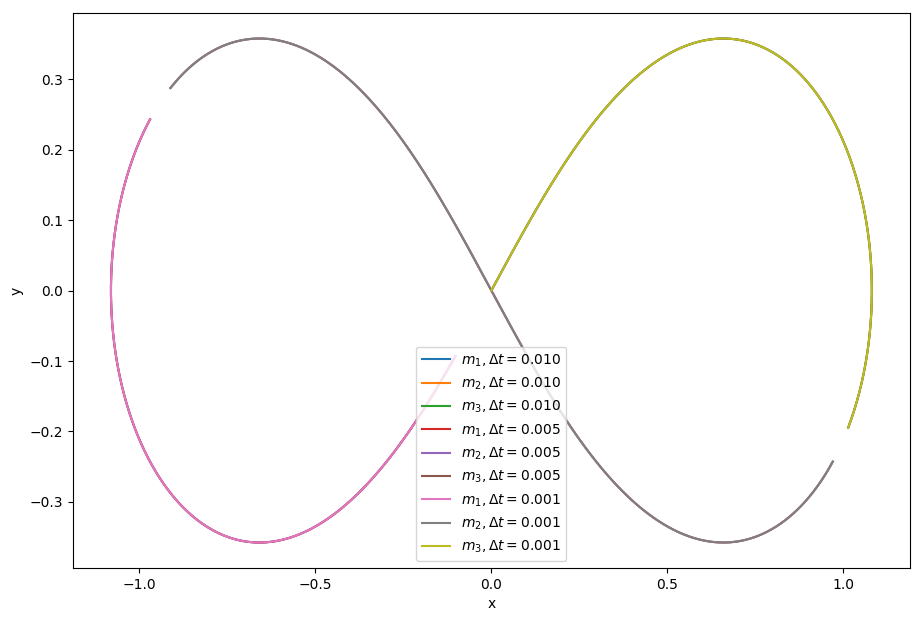
\includegraphics[width=\paperwidth]{3-21-plot}
                \caption{plot of all 3 masses and 3 different stepsizes}
            \end{figure}
        \end{landscape}
        
        
\end{document}
